\documentclass[12pt, letterpaper, twoside]{article}
\usepackage{nopageno,epsfig, amsmath, amssymb}
\usepackage{physics}
\usepackage{mathtools}
\usepackage{hyperref}
\usepackage{xcolor}
\hypersetup{
    colorlinks,
    linkcolor={blue},
    citecolor={blue},
    urlcolor={blue}
}
\usepackage{empheq}
\usepackage{wrapfig}

\usepackage[letterpaper,
            margin=0.8in]{geometry}

\newcommand{\psetnum}{6}
\newcommand{\class}{ASTR 597A - Rubin Observatory and LSST}

\newcommand{\tomtitle}{
    \noindent {\LARGE \fontfamily{cmr}\selectfont \textbf{\class}} \hfill \\[1\baselineskip]
    \noindent {\large \fontfamily{cmr}\selectfont Problem Set \psetnum \hfill \textsc{Tom Wagg}}\\[0.5\baselineskip]
    {\fontfamily{cmr}\selectfont \textit{\today} \hfill Collaborators: David \& Tobin}\\[2\baselineskip]
}

\title{\class : Week \psetnum}
\author{\textbf{Tom Wagg}}

\newcommand{\question}[1]{{\noindent \it #1}}
\newcommand{\answer}[1]{
    \par\noindent\rule{\textwidth}{0.4pt}#1\vspace{0.5cm}
}
\newcommand{\todo}[1]{{\color{red}\begin{center}TODO: #1\end{center}}}

% custom function for adding units
\makeatletter
\newcommand{\unit}[1]{%
    \,\mathrm{#1}\checknextarg}
\newcommand{\checknextarg}{\@ifnextchar\bgroup{\gobblenextarg}{}}
\newcommand{\gobblenextarg}[1]{\,\mathrm{#1}\@ifnextchar\bgroup{\gobblenextarg}{}}
\makeatother

\newcommand{\avg}[1]{\left\langle #1 \right\rangle}
\newcommand{\angstrom}{\mbox{\normalfont\AA}}
\allowdisplaybreaks

\begin{document}

\tomtitle{}

\question{\textbf{1. Definition of H}}
\answer{
    Given that $\alpha = 0$ and both $r$ and $\Delta$ must be $1 \unit{au}$, this means that the Observer would need to be in the same location as the Sun (uh oh).
    \begin{center}
        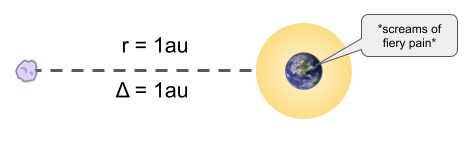
\includegraphics[width=0.5\textwidth]{asteroid_hw_diagram.png}
    \end{center}
}

\question{\textbf{2. Magnitude as a function of distances}}
\answer{
    We currently have an expression for the apparent magnitude as a function of flux. We therefore need an expression of flux in terms of $r$ and $\Delta$. First, let's consider the flux incident on the asteroid. For this we can write our usual expression as
    \begin{align}
        f_{\text{onto-asteroid}} = \frac{L_{\rm \odot}}{4 \pi r^2}
    \end{align}
    Now the asteroid reflects some fraction of this light based on its albedo, $a$. However, this light is emitted in all directions and so we must account for this spreading with a similar factor to the above
    \begin{equation}
        f(r, \Delta) \propto \frac{L_{\rm \odot}}{4 \pi r^2} \cdot \frac{a}{4 \pi \Delta^2},
    \end{equation}
    note that this is only proportional since in reality we'd probably need to integrate over the surface of the asteroid to get the units to work out. But we're about to take a ratio so let's not worry about that. We know that $f_0$ needs to be the value where we get $H$ so
    \begin{equation}
        f_0 = f(1 \unit{au}, 1 \unit{au}) = \frac{L_{\rm \odot} a}{16 \pi^2 \unit{au^4}}
    \end{equation}
    Therefore, we can get the ratio of these two and write the expression for magnitude as
    \begin{equation}
        \boxed{ m = H - 2.5 \log_{10} \qty(\frac{\unit{au^4}}{r^2 \Delta^2}) }
    \end{equation}
}

\clearpage

\question{\textbf{3. Limits}}
\answer{
    First, we are now taking $r = \Delta + 1 \unit{au}$, so we can write the expression for magnitude as
    \begin{equation}
        m = H - 2.5 \log_{10} \qty(\frac{\unit{au^4}}{(\Delta + 1 \unit{au})^2 \Delta^2})
    \end{equation}
    In the case where $\Delta$ is very large, we can ignore the addition of $1 \unit{au}$ and write
    \begin{equation}
        m \approx H - 2.5 \log_{10} \qty(\frac{\unit{au^4}}{\Delta^4})
    \end{equation}
    And so as $\Delta \to \infty$ we find that the magnitudes scales as
    \begin{equation}
        \boxed{ \lim_{\Delta \to \infty} m \propto - \log_{10} \qty( \frac{1}{\Delta^4} ) }
    \end{equation}
    So we can see that the magnitude is scaling with 1/distance$^4$ instead of just 1/distance$^2$ :o That's going to make detecting asteroids rather difficult! The key point here is that the light is \textit{reflected} and so you get this ``spreading out'' of light twice which really attenuates the flux.
}



\end{document}

 